%----------------------------------------------------------------------------
\chapter{Presentation layer}

The frontend is compiled against Java 21, and is built using multiple scenes created using libGDX. The program is completely self-contained, with only a few open-source asset files and fonts required in addition to the declared dependencies -- these are included in the repository.

\section{The rendering pipeline}

\section{Low level graphical challenges}

By using near-machine graphical interfaces, we lose certain simplified operations, for instance the ability to draw complex three-dimensional shapes directly from code. Most graphics cards have certain predispositions about the data they process, and in low-level cases, our program can't guarantee that those rules will be followed. LibGDX provides strong foundations in place of ready-made solutions, which the developer can use to implement or in some cases, disregard the GPU's written or unwritten requests. These include the following examples.

\subsection{Triangulation, ear-clipping algorithm}

Triangles are the most commonly used basic two-dimensional shape that is supported without too many caveats on all platforms. Therefore, it's advisable to reduce any displayed models to a group of them.

One geometrically intuitive division operation is the ear-clipping algorithm. An ear is defined as a triangle made up of three successive vertices of a polygon, where the middle vertex is convex -- in that point, the shape's inner angle must not exceed 180 degrees ($\pi$ raidans).\cite{TriangulationByEarClipping} Areas defined by such triples are guaranteed to be subtractable from the polygon's area, since by definition, they can not contain any holes, removing the need to compensate for empty space. The action can then be repeated on the remaining area, each successive step will result in a new triangular piece; when only three vertices remain, we have achieved our goal of subdivision.

The goal of this algorithm is to create a list of vertex indices that should be connected into triangles, in order to cover the original polygon fully and efficiently. As a useful side effect, this makes calculating the mathematical area trivial as well.

In the case of libGDX, the EarClippingTriangulator class takes care of this common use case. Following OpenGL idioms, the relevant function requests floating point values (vectors decomposed into their axes), and it results in a list of whole number indices -- every group of three defines a triangle to be created.

\begin{lstlisting}[caption=Example usage of the EarClippingTriangulator class]
    val floats = baseNodes.flatMap { listOf(it.x, it.z) }.toFloatArray()
    val triangles: ShortArray
    val triangulator = EarClippingTriangulator()
    triangles = triangulator.computeTriangles(floats)
\end{lstlisting}

\subsection{Winding order}

Many graphical effects - including lighting - require knowledge of the affected faces' normal vectors. In the mathematical sense, this means a direction which is perpendicular to the whole surface, when applied to any contained point of it. %TODO meh 
When observing the side from this particular direction (the vector between the camera and a given point of the face can be represented as a multiple of the normal), the apparent size is at its largest -- in layman's terms, we're seeing the front without any rotations around axes that don't match the normal.

The visibility of a polygon can technically also be treated as an effect. To reduce the number of draw calls, it's advisable to only handle faces that have their intended front side visible from the camera's perspective. By default, OpenGL utilises "back-face culling": the spectator can only see shapes where the order of vertices is counter-clockwise (when plotted in relation to the vector connecting the viewpoint and the weighted center of the polygon). This behaviour is modifiable as follows.

\begin{lstlisting}[caption=Example for changing OpenGL's culling properties through libGDX]
    Gdx.gl.glEnable(GL40.GL_CULL_FACE) //enabling
    Gdx.gl.glCullFace(GL40.GL_BACK) //setting filtered side (rear)
    Gdx.gl.glFront(GL40.CW) //changing the intended winding order to clockwise
\end{lstlisting}

\subsection{Using the main thread}

In contrast to the project's simulation module, the user interface is difficult to parallelise. OpenGL functions are usually not thread-safe, requesting and modifying a single graphical context from multiple areas of code is dangerous and will often lead to crashes.

The graphics library abstracts communication with the operating system and GPU as much as possible. In return it's the developer's responsibility to reduce GPU calls to the absolutely necessary amount. While unique calls are being processed, the GPU can't pass newly created frames to the processor, which is visible as the screen "freezing" -- this is easily observable in the chapter dedicated to performance. 

Aside from frame construction, the program only uses the main graphical thread for creating unique models for each building, as this can't reasonably be done on the CPU.\@I decided against a complex thread-scheduling solution, as the GPU  only receives a heavy workload when creating a new save, or loading an OSM buffer file. When programming, I only had to built on available tools; I used a simple lambda function to obtain the main thread context when needed.

\begin{lstlisting}[caption=Helper function for getting the draw thread]
private suspend fun <T> runOnRenderThread(block: () -> T): T {
        return suspendCoroutine { continuation ->
            Gdx.app.postRunnable {
                continuation.resume(block())
            }
        }
    }
\end{lstlisting}

\section{Implementation}
The program's visual part can be divided into modules. Aside from the interactive, three-dimensional OpenGL scene showcasing the buildings, there exist multiple independent components, aiding user communication.

\section{The main scene}
Buildings are presented in a simplified manner, ignoring any vertical terrain changes. Stylistically, it was inspired by contemporary city building video games (such as SimCity and Cities: Skylines), as well Google Earth.

\begin{figure}[!ht]
    \centering
    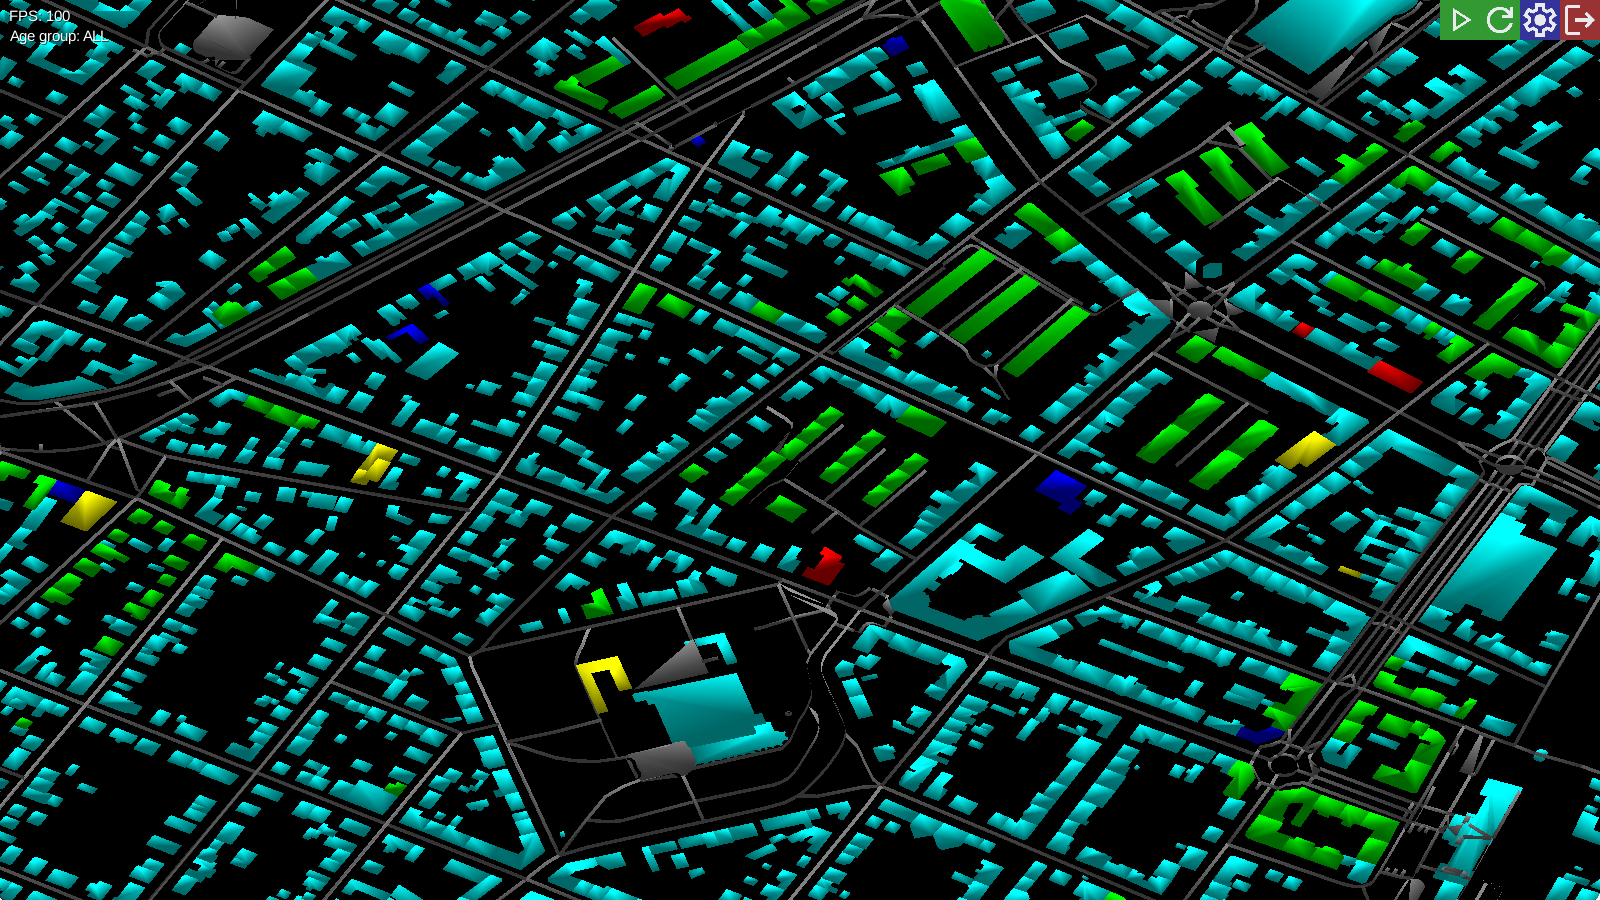
\includegraphics[width=150mm, keepaspectratio]{images/main_graphics_view.png}
    \caption{The main page of the app, with a "false 3D" view}
\end{figure}

\subsection{Custom camera control}

For libGDX scenes, it is possible to inject a single input processing adapter object, or a combination of multiple objects known as a multiplexer. In the recommended starter 3D program\cite{basic3DlibGDX}, the library's creators added the CameraInputController class; this event handler provides mouse-controlled rotation and zooming for its containing scene.

I created my own camera and menu functions based on the public InputAdapter interface. The viewing angle is locked, the user can inspect the image made from backend-sourced data from a fixed top-down perspective. Moving exploits the need for updating the camera every frame; by pressing a navigational button, a certain target amount is added to the handler responsible for the given axis. This number reduces by a certain percentage each frame, zeroing out the value once it gets below a certain threshold.

This results in smooth speed handling, which avoids robotic, sudden direction changes. Since multiple commands may be executed at once, every function that changes the camera's position must be under a mutex (mutually exclusive) lock. Without this, multiple camera location changes cause the currently rendered frame to flicker.
% TODO code section

\
 Egy komplexum, de akár az azt határoló vonalak által leírt poligon is lehet konkáv, így a teljes modellek felépítéséhez a fülvágó algoritmust használtam.

A backend-ről származó adatokból természetesen nem csak az entitások pozíciója, formája lényeges, az OpenStreetMap adathalmaz alapján csoportosíthatók és színezhetők  
